\documentclass[seminarski, times, utf8]{fer}


\usepackage{blindtext}
\usepackage{indentfirst}
\usepackage{graphicx}
\usepackage{float}
\usepackage{subfigure}

%--- PODACI O RADU / THESIS INFORMATION ----------------------------------------

% Naslov na engleskom jeziku / Title in English
\title{Detection and classification of vehicles at intersections for the purpose of optimizing traffic flow }

% Naslov na hrvatskom jeziku / Title in Croatian
\title{Detekcija i klasifikacija vozila na raskrižjima u svrhu optimizacije prometnih tokova}

% Autor / Author
\author{Matija Pavlović}

\voditelj{izv. prof. dr. sc. Tomislav Hrkać}

% Datum rada na engleskom jeziku / Date in English
\date{}

% Datum rada na hrvatskom jeziku / Date in Croatian
\date{}

%-------------------------------------------------------------------------------


\begin{document}


% Naslovnica se automatski generira / Titlepage is automatically generated
\maketitle


%--- SAŽETAK / ABSTRACT --------------------------------------------------------

% Sažetak na hrvatskom
\begin{sazetak}
U ovom istraživanju razvija se sustav za detekciju i klasifikaciju vozila na snimkama prometa u svrhu optimizacije prometnih tokova. Koristimo računalni vid kako bismo analizirali videozapise s prometnih kamera i identificirali vozila prema njihovoj kategoriji (npr. automobili, kamioni, motocikli, tramvaji, autobusi...). Cilj istraživanja je poboljšanje učinkovitosti prometnih raskrižja kroz bolje upravljanje prometnim tokovima temeljenim na stvarnom vremenu. Metodologija obuhvaća kombinaciju tehnika dubokog učenja, kao što su konvolucijske neuronske mreže (CNN), i tradicionalnih algoritama računalnog vida radi precizne detekcije i klasifikacije vozila. Dobiveni podatci će se zatim koristiti u metodama podržanog učenja i evolucijskim algoritmima koji za cilj imaju ubrzanje protoka vozila kroz problematična prometna čvorišta.
\end{sazetak}

\begin{kljucnerijeci}
Računalni vid, detekcija vozila, klasifikacija vozila, optimizacija raskrižja, duboko učenje, konvolucijske neuronske mreže, prometna analiza, prometni tokovi, prometne kamere, podržano učenje, evolucijski algoritmi
\end{kljucnerijeci}

% Sažetak na engleskom
\begin{abstract}
In this research, a system is being developed for the detection and classification of vehicles in traffic footage in order to optimize traffic flow. We utilize computer vision to analyze traffic camera videos and identify vehicles according to their category (e.g., cars, trucks, motorcycles, trams, buses...). The aim of the research is to improve the efficiency of traffic intersections through better real-time traffic flow management. The methodology involves a combination of deep learning techniques, such as convolutional neural networks (CNNs), and traditional computer vision algorithms for precise vehicle detection and classification. The obtained data will then be used in methods such as reinforcement learning and evolutionary algorithms aimed at speeding up vehicle flow through problematic traffic nodes.
\end{abstract}

\begin{keywords}
Computer vision, vehicle detection, vehicle classification, intersection optimization, deep learning, convolutional neural networks, traffic analysis, traffic flows, traffic cameras, reinforcement learning, evolutionary algorithms
\end{keywords}


% Sadržaj se automatski generira / Table of contents is automatically generated
\tableofcontents


%--- UVOD / INTRODUCTION -------------------------------------------------------
\chapter{Uvod}
\label{pog:uvod}
Broj vozila u Hrvatskoj se neprestano povećava. Prema podatcima s Državnog zavoda za statistiku taj broj je 2021. dosegao brojku od 2 385 442 registriranih vozila, što predstavlja povećanje od 3,2\% u odnosu na 2020. godinu. \citep{dzs_website}
Prometnice koje su u Hrvatskoj mahom građene u prošlom stoljeću nisu projektirane za cirkulaciju gore navedene količine vozila što uzrokuje sve češću pojavu prometnih gužvi, a samim time i nezadovoljstvo stanovnika. U ovom seminarskom radu ću iznijeti prijedlog sustava koji, koristeći razne tehnike umjetne inteligencije i strojnog učenja, nastoji optimirati prometne tokove. Predlažu se redom sustavi za detekciju vozila, zatim sustav za klasifikaciju vozila te naposlijetku sustav za optimizaciju prometnih tokova na osnovu koncentracije i tipa vozila na raskrižjima.  


%-------------------------------------------------------------------------------
\chapter{Razrada}
\label{pog:razrada}
U sljedećem poglavlju se detaljno opisuje zamišljeno djelovanje sustava. Razrađuje se potrebna senzorika, djelovi programskog rješenja, algoritmi koji će biti korišteni te relaksirajuće pretpostavke koje će smanjiti kompleksnost problema.
\section{Senzorika}
Primarna prepreka s kojom se susrećemo je dobivanje informacija na osnovu kojih će sustav raditi predikcije. S obzirom da se oslanjamo na snagu algoritama strojnog učenja možemo izbjeći uporabu sofisticiranih senzora i osloniti se na već prisutne kamere kojih primjerice u Zagrebu ima 468 na 156 različitih lokacija.
Detaljnijim proučavanjem specifikacijske brošure jednog od najpopularnijih modela kamere za nadzor prometa "Gatso T series" dolazimo do informacija o sposobnostima uređaja  s kojih je planirano povlačenje podataka. Proizvođačeve specifikacije navode da sustav može istovremeno pratiti brzinu do 12 vozila, naglašena je i visoka fotosenzitivnost senzora, što omogućuje dovoljnu kvalitetu fotografije čak i u uvjetima niske osvjetljenosti.\citep{gatso} Posebno važna stavka je procesorska jedinica koja je sposobna slati sve prikupljene podatke u stvarnom vremenu, ova funkcionalnost uvelike pospješuje mogućnost modela za davanje aktualne i točne konfiguracije prometne mreže.
\section{Detekcija vozila}
Za zadaću detekcije, prebrojavanja i praćenja vozila na raskrižjima koristi se YOLO model koji je u posljednjih nekoliko godina postao središnji sustav za detekciju objekata korišten u raznim primjenama od kojih su industrija, robotika i autonomna vožnja samo neki od primjera. \citep{make5040083}
Razlika između YOLO modela i ostalih alternativa je ta što YOLO model pristupa detekcijskom problemu kroz samo jednu fazu, za razliku od pristupa temeljenih na primjerice R-CNN-ovima. Ovakva arhitektura pospješuje brzinu detekcije uz negativni odraz na točnost. \citep{folio3_yolov8} S obzirom da će brzina obavljanja detekcijske zadaće biti izrazito visoko na ljestvici prioriteta mali gubitak točnosti će biti nužan kompromis koji će uvelike povećati iskoristivost sustava u stvarnom svijetu. Uz integraciju sofisticiranih algoritama za praćenje objekata, primjerice DeepSORT-a, rješava se i druga prepreka u izgradnji sustava za optimizaciju prometnih tokova. Sustav će koristiti \textit{transfer-learning} metodu kako bi dotrenirao već naučeni YOLOv8 na vlastitom skupu podataka. YOLOv8 uključuje i CLI koji omogućuje izrazito jednostavno dotreniranje postojećih modela.
\begin{verbatim}
yolo task=detect \
mode=predict \
model={HOME}/runs/detect/train/weights/best.pt \
conf=0.25 \
source={dataset.location}/test/images
\end{verbatim}
\begin{flushleft}
  \small
Gore navedeni niz naredbi pokreće dotreniranje, dok donji isječak prikazuje korištenje modela za detekciju na ulaznom podatku.
\end{flushleft}
\begin{verbatim}
from ultralytics import YOLO

model = YOLO('yolov8n.pt')
model.predict(
   source=source,
   conf=0.25)
}

\end{verbatim}
 
\begin{figure}[H]
   \centering
   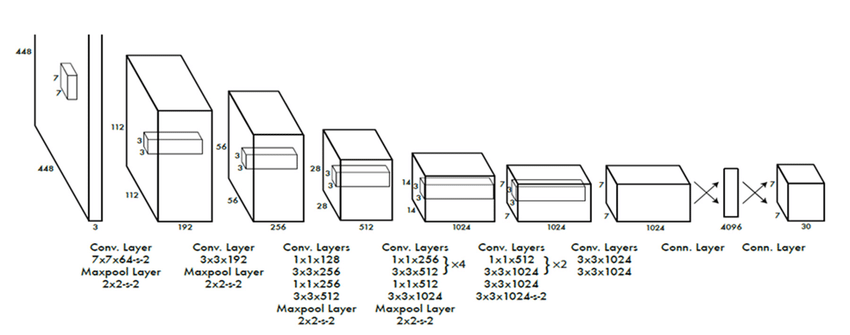
\includegraphics[width=0.7\linewidth]{slike/img2.png}
   \caption{Arhitektura YOLO modela \citep{article}}
   \label{fig:yolo}
\end{figure}
\begin{flushleft}
  \small
  Izvor slike: https://www.researchgate.net/figure/YOLO-architecture-YOLO-architecture-is-inspired-by-GooLeNet-model-for-image\_fig2\_329038564
\end{flushleft}

U odnosu na svoje prethodnike YOLOv8 model donosi razne izmjene. Prva od tih izmjena je \textit{anchor-free} detekcija.
YOLOv4 i YOLOv5 slijede originalnu \textit{anchor} metodu iz YOLOv3. Nedostatci te metode su brojni. Prvo, da bi se postigla optimalna detekcijska izvedba, potrebno je provesti analizu klastera kako bi se odredio optimalni skup sidrišnih točaka prije samog treniranja, što uzrokuje složenije modele manje generalizacijske moći. Drugo, mehanizam sidrišnih točaka povećava složenost detekcije i broj predikcija za svaku sliku. Ovaj problem na brojnim računalnim sustavima predstavlja usko grlo zbog količine potrebnih izračuna te tako smanjuje latenciju sustava.
Detekcijski algoritmi bez sidrišnih točaka se ubrzano razvijaju i pokazali su da performanse takvih detektora mogu postići jednaku razinu točnosti kao i njihovi prethodnici uz značajno smanjenje broja parametara modela. \citep{yolox2021}
Još jedan od iskoraka odabranog modela je uporaba mozaičkog proširenja skupa podataka. Mozaičko proširenje skupa podataka kombinira četiri ili više nasumična primjera u jedinstveni primjer čime se podiže robusnost modela, povećava se iskoristivost skupa za učenje i spriječava prenaučenost. \citep{torres2024yolov8mosaic}
\section{Klasifikacija vozila}
Predloženi sustav još uvijek ne zna o kojem tipu vozila se radi. Ta informacija je izrazito bitna zbog prirode kretanja različitih vozila, autobusi se primjerice kreću sporije od osobnih automobila, teže se prestrojavaju u drugu traku, sporije ubrzavaju i imaju duži zaustavni put. Motocikli pak naprotiv zauzimaju manje prostora i općenito se brže kreću.
Za klasifikacijsku zadaću možemo opet posegnuti za uporabom YOLO modela kao što je pokazano u članku  "Image Classification with YOLOv8" \cite{kalra2024image}. 
\begin{figure}[H]
   \centering
   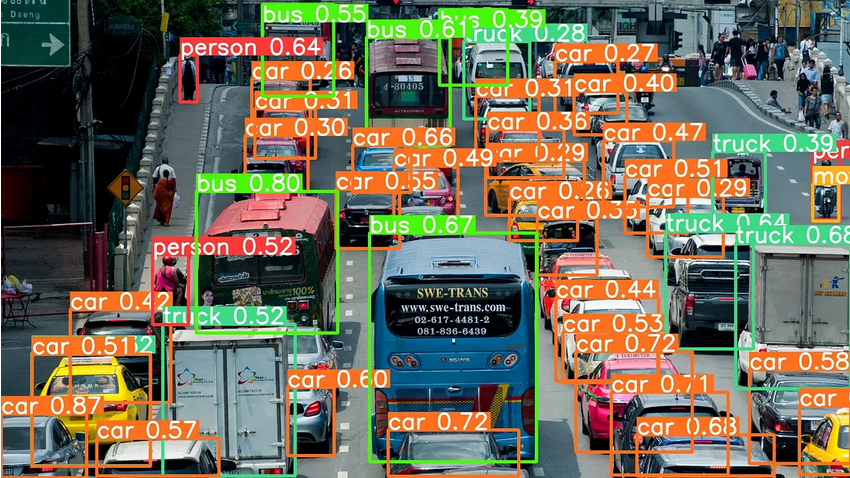
\includegraphics[width=0.7\linewidth]{slike/img1.png}
   \caption{Primjer detekcije i klasifikacije vozila na raskrižjima pomoću YOLO modela}
   \label{fig:detection_and_classification}
\end{figure}

\begin{verbatim}
# import YOLO model
from ultralytics import YOLO

# Load a model
model = YOLO('yolov8n-cls.pt') # load a pretrained model (recommended for training)

# Train the model
model.train(data='/data', epochs=5)
\end{verbatim}
\begin{flushleft}
  \small
  Isječak koda opisuje dodatno treniranje prednaučenog modela 
\end{flushleft}

\section{Algoritam za računanje najvjerojatnijeg sljedećeg čvorišta}
S obzirom da su kamere koje sustav koristi postavljene na fiksne lokacije i pružaju uvijek isti pogled na ciljano raskrižje možemo se koristiti lokacijom vozila na slici kako bi utvrdili prometnu traku u kojoj se vozilo nalazi. Uz pretpostavku da će se većina vozača pridržavati prometnih propisa, informacija o prometnoj traci u kojoj se vozilo nalazi nam daje moguće puteve kojima se pojedino vozilo može kretati. Jedan od načina na koji možemo dobiti informaciju o kretanju i poziciji vozila je primjena DeepSORT algoritma za praćenje objekata. DeepSORT algoritam je relativno jednostavan postupak koji koristi Kalman filtere i "mađarski" algoritam za računanje preklapanja \textit{bounding box-ova}. \citep{wojke2017simple} Algoritam DeepSORT se temelji na četiri osnovna koraka:
\begin{itemize}
	\item Detekcija i ekstrakcija značajki - često YOLO modeli
	\item Kalman filtri za predviđanje stanja
	\item Povezivanje podataka s dubokim metrikama - razlika u odnosu na starije implementacije. "Mađarski" algoritam obavlja povezivanje objekata na različitim okvirima videa koristeći Mahalanobisovu i kosinusnu udaljenost pri izgradnji matrice troška. Ovim korakom dobivamo metriku duboke povezanosti što nam omogućuje praćenje objekta i kroz kraće periode okluzije. 
	\item Upravljanje putanjama - osigurava da sustav zadržava samo aktivne putanje u memoriji. \citep{kouidri2023mastering}
\end{itemize} 
\begin{figure}[H]
   \centering
   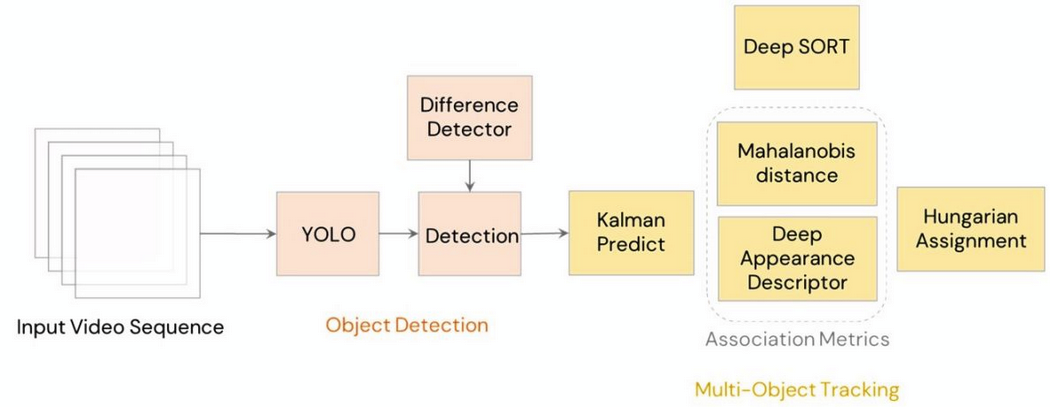
\includegraphics[width=0.7\linewidth]{slike/img5.png}
   \caption{Arhitektura DeepSORT algoritma}
   \label{fig:yolo}
\end{figure}
\begin{flushleft}
  \small
  Izvor slike: https://www.ikomia.ai/blog/deep-sort-object-tracking-guide
\end{flushleft}
Koristeći informacije dobivene iz YOLO modela i algoritma za računanje najvjerojatnijeg sljedećeg raskrižja sada možemo kreirati listu objekata koji predstavljaju pojedino vozilo a sadrže: \textit{bounding-box}
vozila, klasificiranu kategoriju te na osnovu informacija o kretanju vozila njegovo najvjerojatnije sljedeće čvorište.

\section{Optimizacija prometnih čvorišta podržanim učenjem i evolucijskim algoritmima}
Ukoliko prometnu mrežu nekog grada zamislimo kao graf u kojem čvorovi predstavljaju raskrižja a lukovi spajaju križanja koja su povezana prometnicama dobivamo temelj modela nad kojim se vrši optimizacija.
\begin{figure}[H]
   \centering
   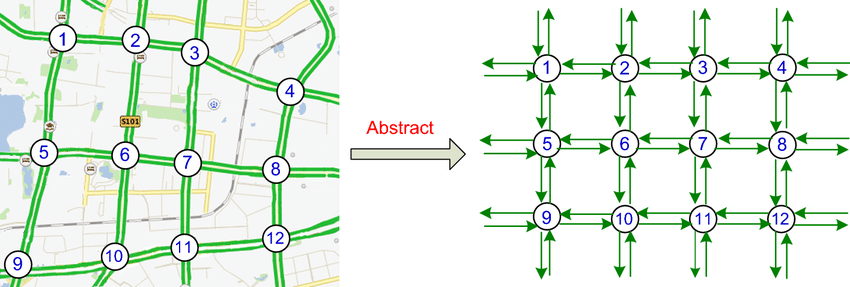
\includegraphics[width=0.7\linewidth]{slike/img4.png}
   \caption{Modeliranje prometne mreže usmjerenim grafom}
   \label{fig:yolo}
\end{figure} Ponovno iz pretpostavke da se većina vozača pridržava prometnih propisa moguće je koristiti udaljenosti duljinu luka (udaljenost dva čvora) i ograničenja brzine na toj dionici kako bi smo dobili vrijeme putovanja vozila između čvorova. Model prometne mreže zatim služi kao okruženje u kojem se podržanim učenjem trenira neuronska mreža kojoj je cilj reducirati količinu zaustavljenih vozila na svakom križanju. U fazi učenja modela podatci koje dobivamo s kamera mogu služiti kako bi smo preciznije modelirali ponašanje modela vozila umjesto da se oslanjamo na neku matematičku funkciju kojom ćemo ostvariti periodične prolaske modela vozila između nasumičnih prometnih čvorišta. Ipak koristeći ovaj postupak moramo paziti da osiguramo dovoljno velik uzorak kako bi model dobio informaciju o sezonalnosti u prometu na dnevnoj, tjednoj, mjesečnoj i godišnjoj razini. Jednom istrenirani model bi kao ulaz primao broj i tip vozila na svakom od raskrižja a kao izlaz bi davao optimalno trajanje crvenog, odnosno zelenog svjetla na svakom od raskrižja. 
\begin{figure}[H]
   \centering
   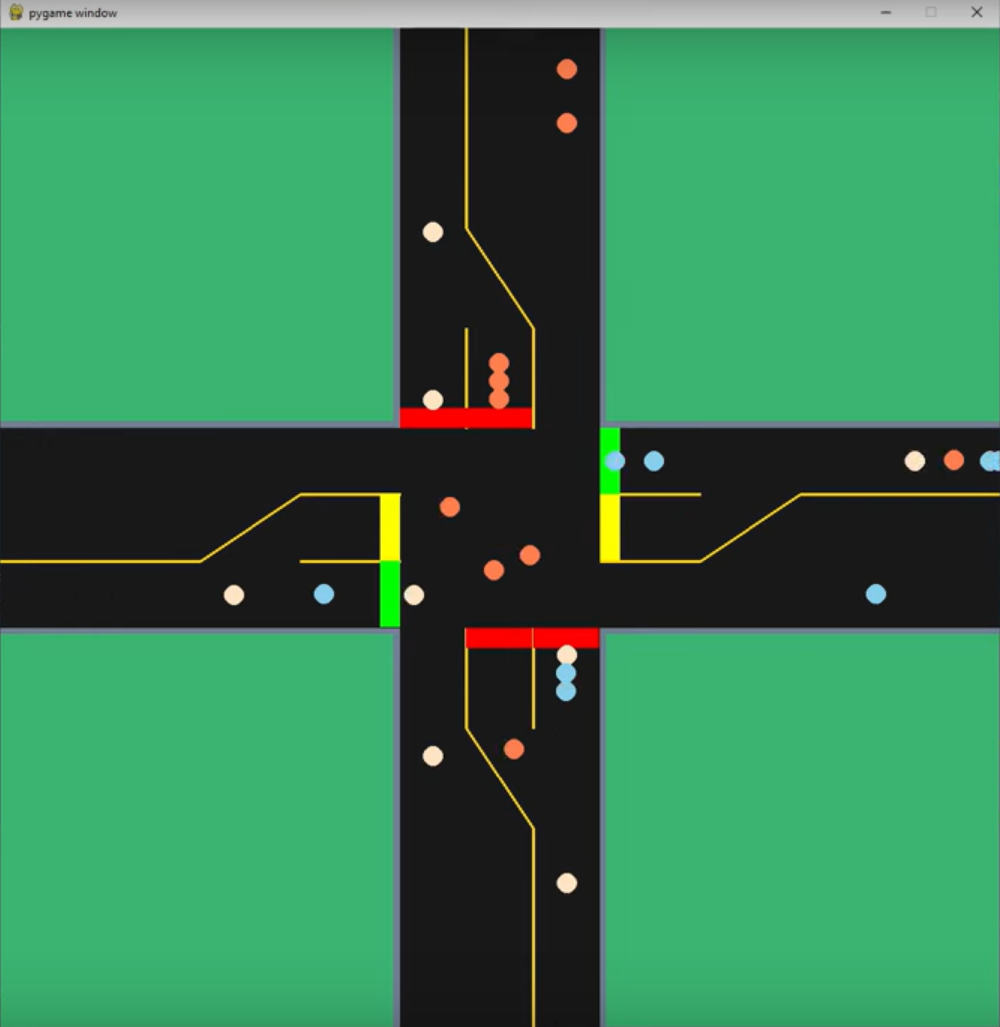
\includegraphics[width=0.7\linewidth]{slike/img3.png}
   \caption{Primjer modela raskrižja pomoću \textit{PyGame library-a}}
   \label{fig:pygame}
\end{figure}
  

%--- ZAKLJUČAK / CONCLUSION ----------------------------------------------------
\chapter{Zaključak}
\label{pog:zakljucak}
U ovom seminarskom radu je iznesen osnovni prijedlog sustava koji integrira algoritme umjetne inteligencije s kamerama koje snimaju prometna raskrižja u svrhu optimizacije toka prometa. Ukoliko bi se ovakav model pokazao uspješnim u regulaciji prometa određivanjem trajanja zelenog i crvenog svjetla te paljenjem dopunskih semafora na raskrižjima, njegova bi uporaba značajno smanjila svakodnevna čekanja u prometnim gužvama. A uz ubrzanje protoka vozila i smanjenje koncentracije vozila na jednom mjestu izvjesno je očekivati i određenu stopu smanjenja prometnih nesreća te unaprijeđenje prometne sigurnosti. Uporaba predloženog sustava bi mogla smaniti i mogućnost ljudske pogreške pri ručnom upravljanju prometnim raskrižjima. Uz uporabu postupaka \textit{online učenja} sustav bi se mogao i konstantno poboljšavati. Implementacija navedene funkcionalnosti ujedno i predstavlja jednu od glavnih fronti budućeg rada na sustavu.


%--- LITERATURA / REFERENCES ---------------------------------------------------

% Literatura se automatski generira / References are automatically generated
% Upiši ime BibTeX datoteke bez .bib nastavka / Enter the name of the BibTeX file without .bib extension
\bibliographystyle{fer} % Choose your bibliography style
\bibliography{literatura}





\end{document}
